\scanpage{28}
$K$ un $\lambda$-anneau $\mathbb Z$-augmenté
\[
\varepsilon:K\mathbin{\text{---}}\mathbb Z
\]
muni d'une famille d'éléments
\[
(E_s)_{s\in S}
\]
satisfaisant
\[
\left\{\begin{array}{l}
\varepsilon(E_s)=n_s\geq0\\
\lambda^i E_s=0\quad\text{si }i>n_s
\end{array}\right.
\]
\[
\lambda^{n_s}E_s\quad\text{inversible}
\]
[\uline{engendrant} $K$]\inserted{et \{stable pour les $\lambda^i$ \inserted{\figure{\begin{tikzpicture}[baseline=(a.base)]
\node[draw,ellipse,inner sep=2pt] (a) {\unsure{pour $+$, pour $\cdot$}};
\draw (a.south west) .. controls +(-.25,-.1) and +(.1,.3) .. ++(-.5,-.65);
\end{tikzpicture}}} et (quand $\unsure{\varepsilon_s}=1$) pour l'inverse\}}, \deleted{\unsure{$\mathcal E$}} et d'un hom
\[
K\xrightarrow{\text{dét}}K^*
\]
tel que
\[
\det(E_s)=\lambda^{n_s}(E_s)
\]
[ce qui détermine dét de façon unique]. \deleted{\unsure{$\}$}}

Une \deleted{chern-}\uline{application de Chern} pour $K$ (muni des structures précédentes) ``dans'' un $A$ gradué, est par définition un \deleted{\illegible{1}}\uuline{hom} de \uuline{$\lambda$-anneaux \unsure{augm.}},
\[
c:K\longrightarrow\widetilde A
\]
[donc définie par sa connaissance sur les $E_s$] \uuline{tel que}
\[
\boxed{c^i(E_s)=0\quad\text{pour }i>n_s}
\]
\diagram{\begin{tikzcd}[column sep=large]
\boxed{c^1(E)=c^1(\text{dét }E)}\arrow[r,bend right=12,dash] & \text{\unsure{conséquence des autres}??}
\end{tikzcd}}

--- conditions qui \unsure{restent vraies} en \unsure{saturant} la famille des $E_s$ par $\lambda^i$ et $\lambda^{n_s}(E_s)^{-1}$ \ldots

Il y a un $A$ \uline{universel},

\margin{\figure{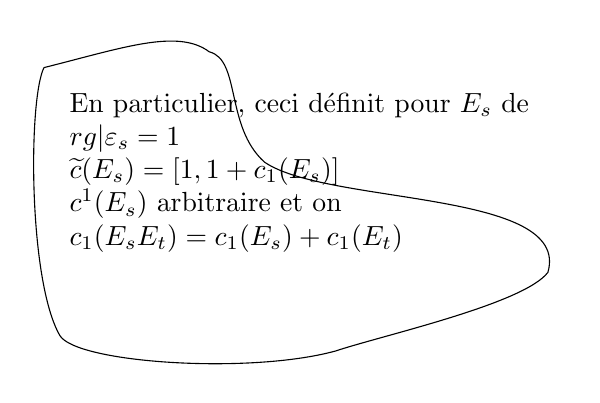
\begin{tikzpicture}[x=1cm,y=1cm]
\node[anchor=north west,align=left,text width=6cm] at (.2,-.1) {En particulier, ceci définit pour $E_s$ de $\unsure{\operatorname{rg}|\varepsilon_s}=1$\par
$\widetilde c(E_s)=[1,1+c_1(E_s)]$\par
$c^1(E_s)$ \unsure{arbitraire} et \deleted{\unsure{on}}\par
$c_1(E_s E_t)=c_1(E_s)+c_1(E_t)$};
\draw (0,.1) .. controls (1,.35) and (1.7,.6) .. (2.1,.3)
 .. controls (2.5,.2) and (2.3,-.65) .. (2.8,-1.1)
 .. controls (3.6,-1.65) and (6.7,-1.45) .. (6.4,-2.5)
 .. controls (6.1,-2.9) and (4.3,-3.3) .. (3.7,-3.5)
 .. controls (2.6,-3.8) and (.4,-3.65) .. (.2,-3.3)
 .. controls (-.2,-2.6) and (-.2,-.3) .. (0,.1);
\end{tikzpicture}}}
\margin{27}
